\documentclass{beamer}
\usetheme{AnnArbor}
\usecolortheme{spruce}
\usepackage{circuitikz}
\usepackage{graphicx}
\usepackage{verbatim}

\title{RAM}
\subtitle{Really Awesome Memory}
\author[CMSC389E]{Akilesh Praveen | CMSC398E}
\institute{UMD}
\date{\today}

\begin{document}

    % title page
    \begin{frame}
        \titlepage
    \end{frame}
    
    % table of contents
    \begin{frame}
        \frametitle{Agenda}
        \tableofcontents
    \end{frame}
    
    \section{Announcements}
    
        \begin{frame}
                \vfill
                \centering
                \begin{beamercolorbox}[sep=8pt,center,shadow=true,rounded=true]{title}
                    \usebeamerfont{title}Announcements\par%
                \end{beamercolorbox}
                \vfill
             \end{frame}
    
        \subsection{Projects 5, 6, and 7}
        
            
            
            \begin{frame}
                \frametitle{Projects 5, 6, 7}
                \begin{itemize}
                    \item Projects 5, 6, and 7 are now released on Piazza
                    \item Relevant instructional material is/will be linked
                    \item They can be done in \textbf{any order}, but I would suggest doing them in order (5, then 6, then 7)
                    \item We already did a lecture on Project 5 and 6, today we'll be talking about \textbf{Project 7}
                    
                \end{itemize}
            \end{frame}
            
            
    \section{Intro + Background}
    
    	\begin{frame}
                \vfill
                \centering
                \begin{beamercolorbox}[sep=8pt,center,shadow=true,rounded=true]{title}
                    \usebeamerfont{title}Intro\par%
                \end{beamercolorbox}
                \vfill
             \end{frame}
    
    		\begin{frame}
    			\frametitle{Intro}
    			\begin{itemize}
    				\item We've built the ALU; the brains of the operation
    				\item Now we need a few more things to take this from just a calculator circuit to an actual computer
    				\begin{itemize}
    					\item Ways to \textbf{store} programs
    					\item Ways to \textbf{interpret} those programs
    					\item Ways to \textbf{execute} those programs
    					\item Ways to \textbf{store data} for those programs while they're executing
    				\end{itemize}
    				\item We're going to use the digital logic circuit theory to build circuits to address all of these! (Projects 5, 6, and 7)
    			\end{itemize}
    		\end{frame}
    		
    		\begin{frame}
    			\frametitle{Intro}
    			
    				\begin{itemize}
    					\item Ways to \textbf{store} programs - \textbf{ROM} \textit{(Project 5)}
    					\item Ways to \textbf{interpret} those programs - \textbf{389E Assembly} \textit{(Project 5)}
    					\item Ways to \textbf{execute} those programs - \textbf{Program Counter} \textit{(Project 6)}
    					\item Ways to \textbf{store data} for those programs while they're executing - \textbf{RAM} \textit{(Project 7)}
    					\item Today, we'll be talking about ways to store data for these programs, using registers of \textbf{RAM}.
    				\end{itemize}
    				
    			
    		\end{frame}
    		
    		\begin{frame}
    			\frametitle{Approach}
    			\begin{itemize}
    				\item Let's figure out our approach to this.
    				\item Right now, we have circuits in place to iterate through the lines of code we're written and provide us with the exact instruction for every line
    				\item Now, while our interpreter circuit (which we have not yet created) is actually executing that code, where will it store the values it calculates?
    				\item We need \textbf{fast-access}, \textbf{modifiable} memory that we can use to store the values that we calculate.
    			\end{itemize}
    		\end{frame}
    		
    		\begin{frame}
    			\frametitle{Approach}
    			\begin{itemize}
    				\item In other words, we need \textbf{registers} for our computer.
    				\begin{itemize}
    					\item Aside: What are registers exactly? Think back to 216 and Assembly
    				\end{itemize}
    				\item At the end of the day, these requirements are pretty much filled out by RAM
    				\item First, we're going to look at the concept of RAM as a whole, and figure out why it's the perfect choice for us here
    				\item Then, we'll talk about implementation in Minecraft
    			\end{itemize}
    		\end{frame}
    		
    		\begin{frame}
    			\frametitle{Overview}
    			{
    			\centering
    			

\tikzset{every picture/.style={line width=0.75pt}} %set default line width to 0.75pt        

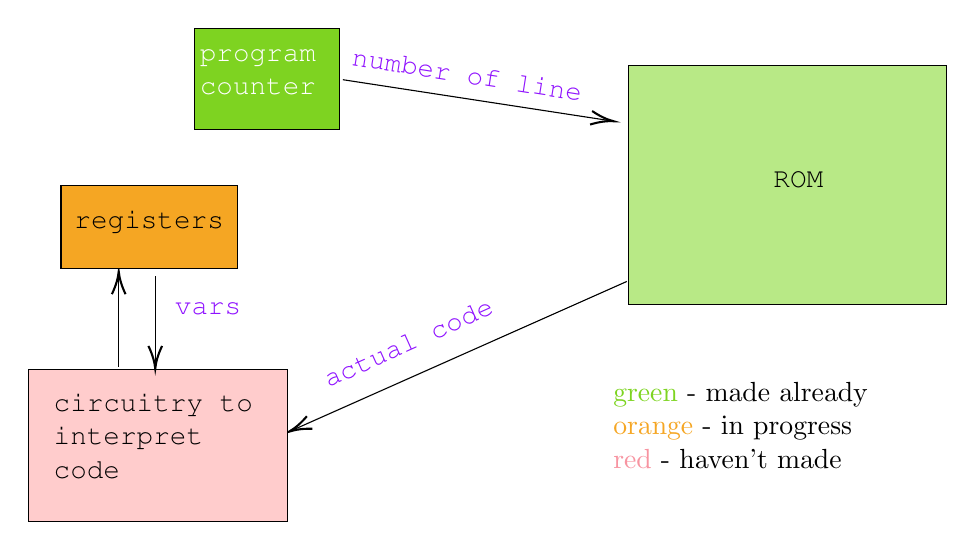
\begin{tikzpicture}[x=0.75pt,y=0.75pt,yscale=-1,xscale=1]
%uncomment if require: \path (0,300); %set diagram left start at 0, and has height of 300

%Shape: Rectangle [id:dp5921038974610358] 
\draw  [fill={rgb, 255:red, 184; green, 233; blue, 134 }  ,fill opacity=1 ] (308.4,56.6) -- (461.4,56.6) -- (461.4,172) -- (308.4,172) -- cycle ;
%Shape: Rectangle [id:dp7682132847374952] 
\draw  [fill={rgb, 255:red, 126; green, 211; blue, 33 }  ,fill opacity=1 ] (99.07,38.8) -- (169.07,38.8) -- (169.07,87.6) -- (99.07,87.6) -- cycle ;
%Straight Lines [id:da4338022631406676] 
\draw    (170.6,63.6) -- (299.02,83.3) ;
\draw [shift={(301,83.6)}, rotate = 188.72] [color={rgb, 255:red, 0; green, 0; blue, 0 }  ][line width=0.75]    (10.93,-3.29) .. controls (6.95,-1.4) and (3.31,-0.3) .. (0,0) .. controls (3.31,0.3) and (6.95,1.4) .. (10.93,3.29)   ;
%Straight Lines [id:da6665272072032727] 
\draw    (307.4,160.8) -- (146.43,232.39) ;
\draw [shift={(144.6,233.2)}, rotate = 336.02] [color={rgb, 255:red, 0; green, 0; blue, 0 }  ][line width=0.75]    (10.93,-3.29) .. controls (6.95,-1.4) and (3.31,-0.3) .. (0,0) .. controls (3.31,0.3) and (6.95,1.4) .. (10.93,3.29)   ;
%Shape: Rectangle [id:dp27632518285076746] 
\draw  [fill={rgb, 255:red, 255; green, 204; blue, 204 }  ,fill opacity=1 ] (19,203.2) -- (143.8,203.2) -- (143.8,276.4) -- (19,276.4) -- cycle ;
%Straight Lines [id:da9669220764176485] 
\draw    (62.6,202) -- (62.6,158) ;
\draw [shift={(62.6,156)}, rotate = 450] [color={rgb, 255:red, 0; green, 0; blue, 0 }  ][line width=0.75]    (10.93,-3.29) .. controls (6.95,-1.4) and (3.31,-0.3) .. (0,0) .. controls (3.31,0.3) and (6.95,1.4) .. (10.93,3.29)   ;
%Straight Lines [id:da14482572171663322] 
\draw    (80.2,158.4) -- (80.2,200.8) ;
\draw [shift={(80.2,202.8)}, rotate = 270] [color={rgb, 255:red, 0; green, 0; blue, 0 }  ][line width=0.75]    (10.93,-3.29) .. controls (6.95,-1.4) and (3.31,-0.3) .. (0,0) .. controls (3.31,0.3) and (6.95,1.4) .. (10.93,3.29)   ;
%Shape: Rectangle [id:dp8111716839726016] 
\draw  [fill={rgb, 255:red, 245; green, 166; blue, 35 }  ,fill opacity=1 ] (34.8,114.4) -- (119.8,114.4) -- (119.8,154.4) -- (34.8,154.4) -- cycle ;

% Text Node
\draw (100.4,47.6) node [anchor=north west][inner sep=0.75pt]   [align=left] {{\fontfamily{pcr}\selectfont \textcolor[rgb]{1,1,1}{program}}\\{\fontfamily{pcr}\selectfont \textcolor[rgb]{1,1,1}{counter}}};
% Text Node
\draw (376.8,106.4) node [anchor=north west][inner sep=0.75pt]   [align=left] {{\fontfamily{pcr}\selectfont ROM}};
% Text Node
\draw (174.9,46.35) node [anchor=north west][inner sep=0.75pt]  [color={rgb, 255:red, 144; green, 19; blue, 254 }  ,opacity=1 ,rotate=-9] [align=left] {{\fontfamily{pcr}\selectfont number of line}};
% Text Node
\draw (158.43,203.75) node [anchor=north west][inner sep=0.75pt]  [rotate=-335.85] [align=left] {{\fontfamily{pcr}\selectfont \textcolor[rgb]{0.56,0.07,1}{actual code}}\\};
% Text Node
\draw (30,213.4) node [anchor=north west][inner sep=0.75pt]   [align=left] {{\fontfamily{pcr}\selectfont circuitry to}\\{\fontfamily{pcr}\selectfont interpret}\\{\fontfamily{pcr}\selectfont code}};
% Text Node
\draw (40,125.4) node [anchor=north west][inner sep=0.75pt]   [align=left] {{\fontfamily{pcr}\selectfont registers}};
% Text Node
\draw (88.4,169.8) node [anchor=north west][inner sep=0.75pt]   [align=left] {{\fontfamily{pcr}\selectfont \textcolor[rgb]{0.56,0.07,1}{vars}}};
% Text Node
\draw (299.6,208.2) node [anchor=north west][inner sep=0.75pt]   [align=left] {\textcolor[rgb]{0.49,0.83,0.13}{green} - made already\\\textcolor[rgb]{0.96,0.65,0.14}{orange} - in progress\\\textcolor[rgb]{0.97,0.58,0.63}{red} - haven't made};


\end{tikzpicture}

    			}
    		\end{frame}
    		
    	\section{RAM as a Concept}
    	
    		\begin{frame}
                \vfill
                \centering
                \begin{beamercolorbox}[sep=8pt,center,shadow=true,rounded=true]{title}
                    \usebeamerfont{title}RAM as a Concept\par%
                \end{beamercolorbox}
                \vfill
             \end{frame}
             
             \begin{frame}
             	\frametitle{What is RAM?}
             	\begin{itemize}
             		\item Known as \textbf{Random Access Memory}
             		\item The quickest memory in the computer that we can pull from and write to
             		\begin{itemize}
             			\item \textit{What a coincidence, that's just what we need!}
             		\end{itemize}
             		\item As such, this is the computer architecture structure that we've decided that our programs will be reading and writing to, reliably quickly, \textit{while they execute}
             		
             	\end{itemize}
             \end{frame}
             
             \begin{frame}
             	\frametitle{What is RAM?}
             	\begin{itemize}
             		\item Keep in mind that we're not just making this stuff up, we're following a general recipe (more on this in the final lecture!)
             		
             		\item Also, Keep in mind that for our case, \textit{RAM} and \textit{Registers} will be used interchangeably
             		\item So, what do the computer gods say about how we should build our RAM? 
             	\end{itemize}
             \end{frame}
             
             \begin{frame}
             	\frametitle{What is RAM?}
             	\begin{itemize}
             		\item \textbf{Volatility:} RAM is only useful when the circuit is powered on, and will lose all the data it's storing when the computer powers off. (For better or for worse)
             		\item \textbf{Access Equality:} It takes the same amount of time to access any address of RAM
             	\end{itemize}
             \end{frame}
             
              \begin{frame}
             	\frametitle{What is RAM?}
             	\begin{itemize}
             		\item \textbf{Volatility:} RAM is only useful when the circuit is powered on, and will lose all the data it's storing when the computer powers off. (For better or for worse)
             		\item \textbf{Access Equality:} It takes the same amount of time to access any address of RAM
             		\begin{itemize}
             			\item How do we achieve this access equality?
             		\end{itemize}
             	\end{itemize}
             \end{frame}
             
             \begin{frame}
             	\frametitle{What is RAM?}
             	\begin{itemize}
             		\item \textbf{Volatility:} RAM is only useful when the circuit is powered on, and will lose all the data it's storing when the computer powers off. (For better or for worse)
             		\item \textbf{Access Equality:} It takes the same amount of time to access any address of RAM
             		\begin{itemize}
             			\item How do we achieve this access equality?
             			\item By leveraging a \textbf{mux} + \textbf{demux} combination, we can efficiently access one of hundreds, thousands, or more memory addresses in a cluster of RAM
             		\end{itemize}
             	\end{itemize}
             \end{frame}
             
             \begin{frame}
             	\frametitle{Aside: Types of RAM (computer world stuff)}
             	\begin{itemize}
             		\item There are two types of RAM in the computer world: \textbf{SRAM} and \textbf{DRAM}
             		\begin{itemize}
             			\item Static RAM and Dynamic RAM
             			\item Static RAM is just circuits, whereas Dynamic RAM is circuits plus a capacitor
             		\end{itemize}
             		\item SRAM is generally faster than DRAM, which is why it is mainly employed in the cache
             		\item DRAM takes up less space, though, (seems counterintuitive, but it's true)
             		\item As such, we use DRAM in the actual RAM chips on our computers (DDR4, DDR5, etc)
             	\end{itemize}
             \end{frame}
             
             \begin{frame}
             	\frametitle{Aside: Types of RAM (computer world stuff)}
             	\begin{itemize}
             		\item Here in CMSC389E, we don't have to worry about silly things like power consumption or storage bandwidth, because our computer is about as smart as a Saguaro Cactus
             		\item As such, we don't need to worry about differentiating between RAM architectures or even building a cache
             		\item Instead, we just need a reliable way for the programs we're executing to be able to read and write to memory while they're running
             	\end{itemize}
             \end{frame}
             
             \begin{frame}
             	\frametitle{RAM Diagram}
             	\begin{itemize}
             		\item Here's how RAM would look in a computer
             		\item As we go over this, try and relate these components to digital logic components you've learned about already
             		\begin{itemize}
             			\item (hint: you know everything you need to know to build this)
             			{
             	\centering
             	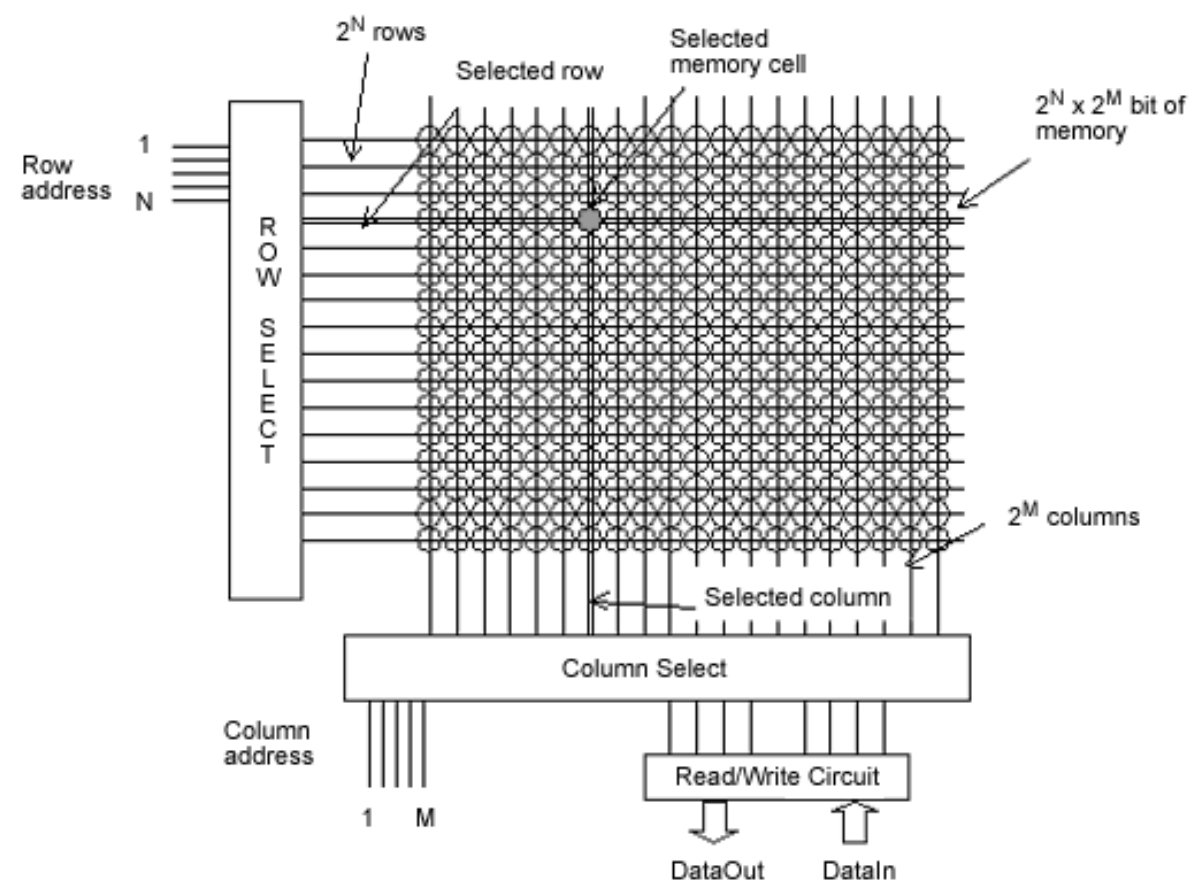
\includegraphics[scale=0.15]{RAM.png} 
             	}
             		\end{itemize}             		             		
             		
             	\end{itemize}
             	
             	
             	
             	
             \end{frame}
             
		\section{RAM in Minecraft}
             
             \begin{frame}
                \vfill
                \centering
                \begin{beamercolorbox}[sep=8pt,center,shadow=true,rounded=true]{title}
                    \usebeamerfont{title}RAM in Minecraft\par%
                \end{beamercolorbox}
                \vfill
             \end{frame}
             
             \begin{frame}
             	\frametitle{What makes RAM different for us?}
             	\begin{itemize}
             		\item Previously on CMSC389E, you worked with ROM, which was \textit{read-only}
             		\item You've also seen the background for basic latches
             		\begin{itemize}
             			\item Remember, latches are just augmented flip-flops. Look back to the 'memory' lecture if you need a refresher.
             		\end{itemize}
             		\item We also talked about using a form of latch-based storage to keep track of the numbers we were counting for our program counter
             		
             	\end{itemize}
             	
             \end{frame}
             
             \begin{frame}
             	\frametitle{What makes RAM different for us?}
             	\begin{itemize}
             		\item Think of this next problem we're tackling as a further exploration of consistent value storage, as a beautiful combination of the last two projects you worked on
             		\item We're going to store data in a similar way to what you've seen in the ROM (using a neat decoder-based technique to \textbf{read} from it)
             		\item We're going to use latches in an intelligent way (similar to what you saw in the program counter project) in order to \textbf{write} data
             	\end{itemize}
             \end{frame}
             
             \begin{frame}
             	\frametitle{What makes RAM different for us?}
             	\begin{itemize}
             		\item Before, you essentially created a singular 'register' that could be added to and subtracted from every cycle. Now, our goal is to do \textbf{two things}
             		\item Remove any extraneous bits from that logical circuit
             		\item Cut that down to a more compact, modular form (we want to put a bunch of RAM together!)
             	\end{itemize}
             \end{frame}
             
             \begin{frame}
             	\frametitle{So What do We Need?}
             	\begin{itemize}
             		\item Let's synthesize this information into an actionable set of requirements
             		\item We need a circuit that \textbf{stores data} for us, that we can easily \textbf{write to} and \textbf{read from}
             	\end{itemize}
             \end{frame}
             
             \begin{frame}
             	\frametitle{So What do We Need?}
             	\begin{itemize}
             		\item Let's synthesize this information into an actionable set of requirements
             		\item We need a circuit that \textbf{stores data} for us, that we can easily \textbf{write to} and \textbf{read from}
             		\item We need to be able to access all the \textbf{numerous} addresses in that circuit as \textbf{efficiently as possible}
             	\end{itemize}
             \end{frame}
             
             \begin{frame}
             	\frametitle{So What do We Need?}
             	\begin{itemize}
             		\item Let's synthesize this information into an actionable set of requirements
             		\item We need a circuit that \textbf{stores data} for us, that we can easily \textbf{write to} and \textbf{read from}
             		\item We need to be able to access all the \textbf{numerous} addresses in that circuit as \textbf{efficiently as possible}
             		\begin{itemize}
             			\item Optimally, we want to request and address in binary, and be able to perform a R/W operation on that particular register
             		\end{itemize}
             		
             	\end{itemize}
             \end{frame}
             
             \begin{frame}
             	\frametitle{So What do We Need?}
             	\begin{itemize}
             		\item Let's synthesize this information into an actionable set of requirements
             		\item We need a circuit that \textbf{stores data} for us, that we can easily \textbf{write to} and \textbf{read from}
             		\item We need to be able to access all the \textbf{numerous} addresses in that circuit as \textbf{efficiently as possible}
             		\begin{itemize}
             			\item Optimally, we want to request and address in binary, and be able to perform a R/W operation on that particular register
             		\end{itemize}
             		\item Take a moment to think about which components we'll need
             	\end{itemize}
             \end{frame}
             
             \begin{frame}
             	\frametitle{So What do We Need?}
             	\begin{itemize}
             		\item Let's list out the circuits that we've talked about in order to get this done.
             	\end{itemize}
             	{
             	\centering
             	

\tikzset{every picture/.style={line width=0.75pt}} %set default line width to 0.75pt        

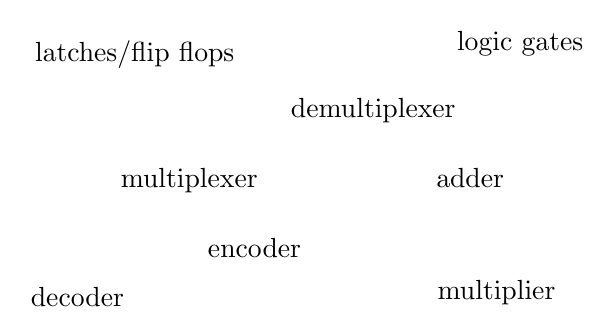
\begin{tikzpicture}[x=0.75pt,y=0.75pt,yscale=-1,xscale=1]
%uncomment if require: \path (0,300); %set diagram left start at 0, and has height of 300


% Text Node
\draw (134,105.33) node [anchor=north west][inner sep=0.75pt]   [align=left] {multiplexer};
% Text Node
\draw (216,71.33) node [anchor=north west][inner sep=0.75pt]   [align=left] {demultiplexer};
% Text Node
\draw (90.67,162.33) node [anchor=north west][inner sep=0.75pt]   [align=left] {decoder};
% Text Node
\draw (286,105.33) node [anchor=north west][inner sep=0.75pt]   [align=left] {\textcolor[rgb]{0,0,0}{adder}};
% Text Node
\draw (176,139) node [anchor=north west][inner sep=0.75pt]   [align=left] {encoder};
% Text Node
\draw (92.67,44) node [anchor=north west][inner sep=0.75pt]   [align=left] {\textcolor[rgb]{0,0,0}{latches/flip flops}};
% Text Node
\draw (286.67,159) node [anchor=north west][inner sep=0.75pt]   [align=left] {multiplier};
% Text Node
\draw (296,39) node [anchor=north west][inner sep=0.75pt]   [align=left] {logic gates};


\end{tikzpicture}

             	}
             \end{frame}
             
             \begin{frame}
             	\frametitle{So What do We Need?}
             	\begin{itemize}
             		\item Here are some circuits that come to mind
             	\end{itemize}
             	
             	{
             	\centering
             	

\tikzset{every picture/.style={line width=0.75pt}} %set default line width to 0.75pt        

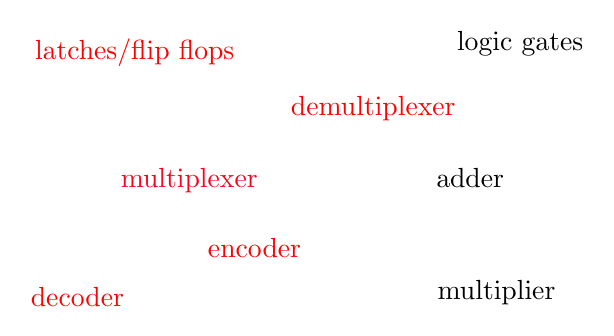
\begin{tikzpicture}[x=0.75pt,y=0.75pt,yscale=-1,xscale=1]
%uncomment if require: \path (0,300); %set diagram left start at 0, and has height of 300


% Text Node
\draw (134,105.33) node [anchor=north west][inner sep=0.75pt]   [align=left] {\textcolor[rgb]{1,0,0.12}{multiplexer}};
% Text Node
\draw (216,70.33) node [anchor=north west][inner sep=0.75pt]   [align=left] {\textcolor[rgb]{1,0,0}{demultiplexer}};
% Text Node
\draw (90.67,162.33) node [anchor=north west][inner sep=0.75pt]   [align=left] {\textcolor[rgb]{1,0,0}{decoder}};
% Text Node
\draw (286,105.33) node [anchor=north west][inner sep=0.75pt]   [align=left] {\textcolor[rgb]{0,0,0}{adder}};
% Text Node
\draw (176,139) node [anchor=north west][inner sep=0.75pt]   [align=left] {\textcolor[rgb]{1,0,0}{encoder}};
% Text Node
\draw (92.67,43) node [anchor=north west][inner sep=0.75pt]   [align=left] {\textcolor[rgb]{1,0,0}{latches/flip flops}};
% Text Node
\draw (286.67,159) node [anchor=north west][inner sep=0.75pt]   [align=left] {multiplier};
% Text Node
\draw (296,39) node [anchor=north west][inner sep=0.75pt]   [align=left] {logic gates};


\end{tikzpicture}

             	}
             \end{frame}
             
             
	\section{Implementation Details}
	
		\begin{frame}
                \vfill
                \centering
                \begin{beamercolorbox}[sep=8pt,center,shadow=true,rounded=true]{title}
                    \usebeamerfont{title}Implementation Details\par%
                \end{beamercolorbox}
                \vfill
        \end{frame}
        
        \begin{frame}
        		\frametitle{Implementation Details}
        		\begin{itemize}
        			\item Ok, so we've got a general idea of how we want to build our RAM
        			\item We've seen a picture of how it's done on computers
        			\item We also know the general components that we want to be employing in this implementation
        			\item \textbf{Big Question:} How will \textit{we} implement it?
        		\end{itemize}
        \end{frame}
        
        \begin{frame}
        		\frametitle{D Flip Flop}
        		\begin{itemize}
        			\item We're implementing SRAM (No need for capacitor here)
        			\item We'll be using D Flip Flops
        			\begin{itemize}
        				\item The D in this case stands for data
        			\end{itemize}
        			\item Think of a D Flip Flop as an augmented version of the SR Flip Flops we learned about earlier\\
        			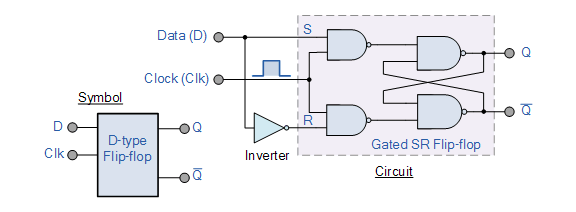
\includegraphics[scale=0.5]{dflipflop} 
        		\end{itemize}
        \end{frame}
        
        \begin{frame}
        		\frametitle{D Flip Flop}
        		\begin{itemize}
        			\item It's basically our old Flip Flop, with an added special feature- we're making sure the same signal isn't fed in from both S and R
        			\item If this is confusing for you, just understand that it's a very cool way to use flip flops (latches) to store data
        			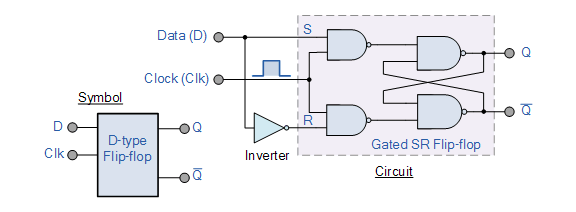
\includegraphics[scale=0.5]{dflipflop} 
        		\end{itemize}
        \end{frame}
        
        \begin{frame}
        		\frametitle{D Flip Flops}
        		\begin{itemize}
        			\item Just like before, each Flip Flop can be seen as one \textbf{bit} of memory
        			\begin{itemize}
        				\item That is, each of these fancy circuits can store either a 1 or a 0
        			\end{itemize}
        		\end{itemize}
        \end{frame}
        
        \begin{frame}
        		\frametitle{D Flip Flops}
        		\begin{itemize}
        			\item Just like before, each Flip Flop can be seen as one \textbf{bit} of memory
        			\begin{itemize}
        				\item That is, each of these fancy circuits can store either a 1 or a 0
        			\end{itemize}
        			\item We're going to need a lot more of these!
        		\end{itemize}
        \end{frame}
        
        \begin{frame}
        		\frametitle{D Flip Flops}
        		\begin{itemize}
        			\item Just like before, each Flip Flop can be seen as one \textbf{bit} of memory
        			\begin{itemize}
        				\item That is, each of these fancy circuits can store either a 1 or a 0
        			\end{itemize}
        			\item We're going to need a lot more of these!
        			\item Okay, let's assume we now have a ton of these bad boys, all laid out in some sort of array or matrix.
        			\item How would we efficiently be able to access the ones we want?
        		\end{itemize}
        \end{frame}
        
        \begin{frame}
        		\frametitle{D Flip Flops}
        		\begin{itemize}
        			\item Just like before, each Flip Flop can be seen as one \textbf{bit} of memory
        			\begin{itemize}
        				\item That is, each of these fancy circuits can store either a 1 or a 0
        			\end{itemize}
        			\item We're going to need a lot more of these!
        			\item Okay, let's assume we now have a ton of these bad boys, all laid out in some sort of array or matrix.
        			\item How would we efficiently be able to access the ones we want?
        			\begin{itemize}
        				\item \textbf{Hint:} Remember when we talked about efficient memory addressing in a previous lecture?
        			\end{itemize}
        		\end{itemize}
        \end{frame}
        
        \begin{frame}
        		\frametitle{MUX \& DEMUX}
        		\begin{itemize}
        			\item To get the specific memory address we want, we will use a demux
        			\item We're going to use an array for simplicity's sake
        			\item Plus, there's another very cool reason we want to build these RAM blocks in order...
        			
        		\end{itemize}
        \end{frame}
        
        \begin{frame}
        		\frametitle{Sequential Access}
        		\begin{itemize}
        			\item What if we want to pull more than just a singular bit from RAM?
        			\item In fact, this is a common problem in the real world- that's why RAM has \textbf{block sizes}
        			\item If your block size is $4$, and you want to pull the block starting at $n$, all you need to do is use a counter
        			\begin{itemize}
        				\item Then you'll be able to pull from $n$, $n+1$, $n+2$, and $n+3$
        			\end{itemize}
        			\item \textbf{Aside:} Most computers distinguish clearly between RAM and registers, but we're going to splay the definition a little, just for our convenience
        		\end{itemize}
        \end{frame}
        
        \begin{frame}
        		\frametitle{General Architecture}
        		\begin{itemize}
        			\item \textbf{Aside}: We're straying from real world architecture choices a bit, but don't forget that this is still a game :)
        			\item We don't have to concern ourselves with the nuances of electronics, nor do we have the same spatial limitations of the real world
        			\item What we do have is limited time and workload expectation, so that's what we're forced to work with
        			\item \textbf{TL;DR} we made things easier when making certain architectural choices. You are still building a functional computer, albeit a \textit{very} simple one.
        		\end{itemize}
        \end{frame}
        
        
    \section{Final Project}
    
    		\begin{frame}
                \vfill
                \centering
                \begin{beamercolorbox}[sep=8pt,center,shadow=true,rounded=true]{title}
                    \usebeamerfont{title}Final Project\par%
                \end{beamercolorbox}
                \vfill
        \end{frame}
		
	
	
	\section{Demo}
	
	
		\begin{frame}
                \vfill
                \centering
                \begin{beamercolorbox}[sep=8pt,center,shadow=true,rounded=true]{title}
                    \usebeamerfont{title}Demo\par%
                \end{beamercolorbox}
                \vfill
        \end{frame}
    	
    	
    		
    		
		
            
        
   	
\end{document}
